\documentclass{article}
\usepackage{graphicx}
\usepackage{tikz}
\usepackage[active,tightpage]{preview}
\PreviewEnvironment{tikzpicture}
\setlength\PreviewBorder{10pt}%

% Graphical representation of unboundedness.
% Model that starts in a small radius.
% Then you run the simulation and the model expands outward.

\begin{document}
\begin{tikzpicture}
    \node[] (before) at (0,0)
        {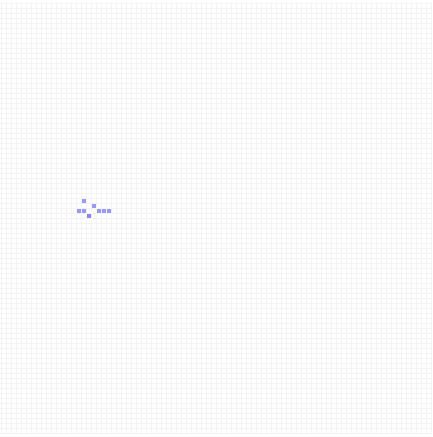
\includegraphics[width=5cm]{before.png}};

    \node[] (after) at (8,0)
        {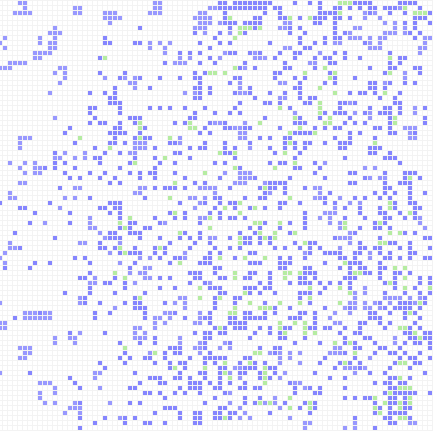
\includegraphics[width=5cm]{after.png}};

    \draw[->,thick] (before.east) -- (after.west)
        node[midway,anchor=south] {run simulation};

    \draw[magenta] (2,-2.9) node[anchor=east]{start in small radius};
    \draw[magenta] (10.3,-2.9) node[anchor=east]{grows outwards unboundedly};
\end{tikzpicture}
\end{document}
